\documentclass{tufte-handout}
\usepackage{amsmath}
\usepackage{mathpazo}

\usepackage{tikz}
\usetikzlibrary{chains}
% Define style for nodes
\tikzstyle{every node}=[circle, draw, fill=white,
                        inner sep=0pt, minimum width=9pt,font=\footnotesize\sf]
\tikzstyle{every picture}= [scale=.5,baseline=(current bounding box.center)]
\usetikzlibrary{automata}
\usetikzlibrary{patterns}
\usepackage{booktabs}
\usepackage{siunitx}
\IfFileExists{vc.tex}{\input{vc.tex}}{\newcommand\GITAuthorDate{no git info found}\newcommand\GITAbrHash{-}}  % For version control

\title{Heaps}
\author{}
\date {\GITAuthorDate, rev. \GITAbrHash}

\begin{document}
\maketitle
%\section{}
%\subsection{}

\begin{abstract}
\end{abstract}

\section{\textbf{Description}}
  This assignment helps test your knowledge about linked-lists, stacks, union-find and heaps. 
  
  \medskip Question 1 and 2 contain previous exam questions. An additional goal with these is to familiarize you with the exam notation. Question 3 and 4 are from the book, and similar questions will be asked on the exam.
  
  \medskip Do not be discouraged if you find Question 4 challenging. The hints on the last page should help point you in the right direction. We will also go through a similar question, 2.4.29, in the exercise class this week. It is obviously possible to solve the problem without considering 2.4.29, it is just meant as a help.

\section{\textbf{Deliverable}}
1. A PDF with your answers.

\medskip You do not need to write code for any of these questions, although you are welcome to provide pseudocode as part of your answer if you want to. You should be able to answer Question 3 in two or three sentences. Question 4 will require a bit more, and a drawing might be helpful (but is not required).


\section{\textbf{Question 1}: from exam 150819 3a}
Insert the keys {\tt 1 3 6 2 4 5} in that order into a heap. Draw the result.

\section{\textbf{Question 2}: from exam 170815 3a, e, f}
\begin{description}
  \item[(3a)] 
    Consider a Stack $S$, implementated as a linked list.
    Beginning with an empty data structure, assume I called
    {\tt S.push("World");} 
    {\tt S.push("World");} 
    {\tt S.pop();}, and 
    {\tt S.push("Hello");}.
    How does the data structure look after these operations?

    (a)
    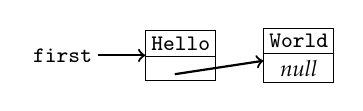
\begin{tikzpicture}
      \node[draw = none,rectangle,inner sep = 2pt] (first) at (-3,0) {{\tt first}};
      \node[rectangle split, rectangle split parts = 2, inner sep = 2pt]
	(hello) { {\tt Hello} \nodepart{second} };
      \node[rectangle split, rectangle split parts = 2, inner sep = 2pt]
	(world) at (3,0)
	{ {\tt World} \nodepart{second} {\rm\em null}};
	\draw[->, thick] (first)--(hello);
	\draw[->, thick] (hello.second)--(world);
      \end{tikzpicture}

     (b)
    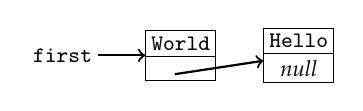
\begin{tikzpicture}
      \node[draw = none,rectangle,inner sep = 2pt] (first) at (-3,0) {{\tt first}};
      \node[rectangle split, rectangle split parts = 2, inner sep = 2pt]
	(world) { {\tt World} \nodepart{second} };
      \node[rectangle split, rectangle split parts = 2, inner sep = 2pt]
	(hello) at (3,0)
	{ {\tt Hello} \nodepart{second} {\rm\em null}};
	\draw[->, thick] (first)--(world);
	\draw[->, thick] (world.second)--(hello);
    \end{tikzpicture}

    (c)
    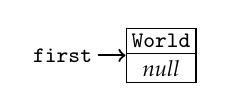
\begin{tikzpicture}
      \node[draw = none,rectangle,inner sep = 2pt] (first) at (.5,0) {{\tt first}};
      \node[rectangle split, rectangle split parts = 2, inner sep = 2pt]
	(world) at (3,0)
	{ {\tt World} \nodepart{second} {\rm\em null}};
	\draw[->, thick] (first)--(world);
    \end{tikzpicture}

    (d)
    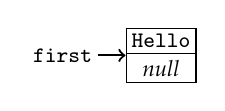
\begin{tikzpicture}
      \node[draw = none,rectangle,inner sep = 2pt] (first) at (.5,0) {{\tt first}};
      \node[rectangle split, rectangle split parts = 2, inner sep = 2pt]
	(hello) at (3,0)
	{ {\tt Hello} \nodepart{second} {\rm\em null}};
	\draw[->, thick] (first)--(hello);
    \end{tikzpicture}


  \medskip\item[(3e)]
  Consider a quick-find implementation of Union--Find with 5 elements.
  After some operations, the internal data structure looks like this:

  \begin{tabular}{ccccc}
    \multicolumn{5}{c}{\tt id[]}\\
  0 & 1 & 2 & 3 & 4 \\ 	\hline
  0 & 1 & 2 & 2 & 4 
  \end{tabular}

  Assume we now union elements 2 and 4. How does the resulting data structure look?

  \medskip\item[(3f)]
    In which sense is it Quick-union better than Quick-find? 
      \begin{enumerate}
        \item The union operation is asymptotically faster. 
        \item The amortized complexity of find is asymptotically faster. 
        \item It can compute a minimum forest. 
        \item It uses less space.
      \end{enumerate}
\end{description}

\section{\textbf{Question 3}: [SW] 2.4.27 Find the minimum}
Consider MaxPQ defined on page 309 of the book. Describe concisely which alterations you would make to add a min() method that uses constant time and constant extra space.


\section{\textbf{Question 4}: [SW] 2.4.30 Dynamic median-finding}
Design a data type that supports the following operations:
\begin{itemize}
    \item insert in logarithmic time
    \item find the median in constant time
    \item delete the median in logarithmic time
\end{itemize}

If you get stuck, consider the hints on the next page. How many hints did you need? Was the solving of 2.4.29 in class helpful?
\newpage
\section{\textbf{Hints for Question 4}}
\begin{enumerate}
    \item Draw the numbers "1, 3, 5, 7, 9" on a line. 5 is obviously the median. Add the numbers "11, 13, 15" to the right and notice how the median changes. Now add the numbers "-1, -3" to the left and update the median as you do. Do you notice a helpful pattern?
    \item Look at your line of numbers, and consider using two heaps, a min-heap and max-heap to keep track of the numbers.
    \item Consider keeping track of and balancing the sizes of each heap as you add and remove elements.
\end{enumerate}


\end{document}